\documentclass{article}

\usepackage{booktabs}
\usepackage{graphicx}
\usepackage{caption}
\usepackage{subcaption}

\graphicspath{{../dev/}}

\title{Strategy Analysis: Progressive Entry with 5\% Stop Wins}
\author{Ivan Anich}

\begin{document}
\maketitle

Here is my analysis of a set of progressive entry strategies with stop wins. These strategies feature high win percentages and low average losses: they are a consistent source of small wins. 

I analyzed stop losses as well, but ultimately chose to not include them. Tight stop losses were not a profitable tactic. The best use seemed to be a very high stop loss, such that catastrophic losses were prevented without prematurely turning too many winners into losers. That being said, the two largest losses found in backtesting were 48\% and 30\%, both occurring in strategy 4, which is a strategy I do not recommend regardless.

\section{Signal}

The signal analyzed is a rise of 20\% from the open, with a previous close between \$1 and \$2. 

\section{Strategy 1: Unlimited Entries, 5\% Stop Win Relative to Average Cost, Exit at 11}

\begin{table}
\caption{Performance of Strategy 1: Unlimited Entries, 5\% Stop Win Relative to Average Cost, Exit at 11}
\center{Overall}
\\[2ex]
\begin{tabular}{lcccc}
\hline
         &  0.1   &  0.9   & median & average   \\
\midrule
\midrule
constant & 0.0152 & 0.0500 & 0.0500 & 0.0410    \\
         & (inf)  & (inf)  & (inf)  & (0.0027)  \\
N        & 65     & 65     & 65     & 65        \\
Win rate & 0.92   & 0.92   & 0.92   & 0.92      \\
\hline
\end{tabular}

\center{Winners}
\\[2ex]
\begin{tabular}{lcccc}
\hline
         &  0.25  &  0.75  & median & average   \\
\midrule
\midrule
constant & 0.0500 & 0.0500 & 0.0500 & 0.0463    \\
         & (inf)  & (inf)  & (inf)  & (0.0014)  \\
N        & 60     & 60     & 60     & 60        \\
Win rate & 0.92   & 0.92   & 0.92   & 0.92      \\
\hline
\end{tabular}

\center{Losers}
\\[2ex]
\begin{tabular}{lcccc}
\hline
          &  0.25  &  0.75  & median & average   \\
\midrule
\midrule
constant  & 0.0025 & 0.0311 & 0.0280 & 0.0228    \\
          & (nan)  & (nan)  & (nan)  & (0.0093)  \\
N         & 5      & 5      & 5      & 5         \\
Loss rate & 0.08   & 0.08   & 0.08   & 0.08      \\
\hline
\end{tabular}
\label{tab_strat_1}
\end{table}

I think of this strategy as the baseline for the family of strategies involving progressive entries and stop wins. The strategy is as follows. The first entry into a trade occurs when a stock exhibits the above signal. The size of this entry is some amount \$X. Each time the stock rises another 5\%, it is entered into again with a position size double that of the last entry: so the first entry is \$X, second is 2*\$X, third 4*\$X, etc. If at any point the stock falls to 5\% below the average cost of the trade, a stop win is executed and profits are taken. If the stock has one entry, average cost is \(1.2*open\) and a stop win is triggered at \(1.15*open\); if it has 3 entries, average cost is \(1.27*open\) and a stop win is triggered at \(1.22*open\). Note that the stop win trails the \textit{current} average cost, such that it always guarantees 5\% profits relative to the current average cost given the number of entries a trade has. Trades are only entered between the day's open and 11 a.m.

Table \ref{tab_strat_1} reports strategy 1's performance, which is very good. It's \textbf{weighted expected return is 5.0\%}, although it appears this is mainly driven by a single trade that won with 20 entries (see figure \ref{hist_strat_1}). It is very expensive to buy all of the possible entries a trade can have. That being said, the use of stop wins means that trades have fewer entries than they would have otherwise: all but 1 trade have 9 or fewer entries. The dominating features of this strategy are its win percentage, 92\%, and its small average loss of 2.3\%. These speak to how low risk this strategy can be, if you are willing to pay for up to 9 entries. A trade with 9 entries has a total position size of 511*\$X.

\begin{figure}
	\center{Histogram of Trades by Number of Entries for Unlimited Entries, 5\% Stop Win Relative to Average Cost, Exit at 11}
	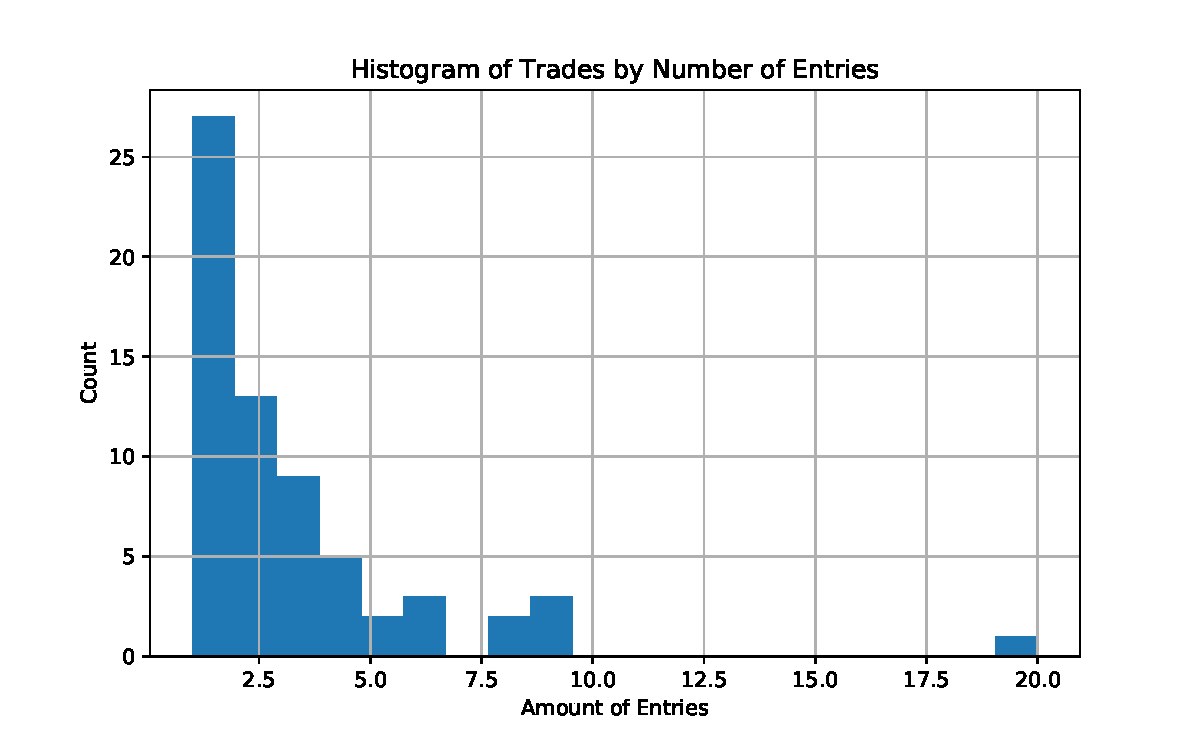
\includegraphics[width=\textwidth]{prog_entry_stop_win_hist.pdf}
	\caption{This table shows counts of the numbers of trades that had a certain amount of entries. For example, it says that around 27 trades had only 1 entry, and that around 3 trades had 9 entries (fist entry and 8 adds).}
	\label{hist_strat_1}
	\end{figure}
\pagebreak

\section{Strategy 2: Max 3 Entries, 5\% Stop Win Relative to Average Cost, Exit at 11} 


\begin{table}
\caption{Performance of Strategy 2: Max 3 Entries, 5\% Stop Win Relative to Average Cost, Exit at 11}
\center{Overall}
\\[2ex]
\begin{tabular}{lcccc}
\hline
         &   0.1   &  0.9   & median & average   \\
\midrule
\midrule
constant & -0.0280 & 0.0500 & 0.0500 & 0.0318    \\
         & (inf)   & (inf)  & (inf)  & (0.0052)  \\
N        & 65      & 65     & 65     & 65        \\
Win rate & 0.86    & 0.86   & 0.86   & 0.86      \\
\hline
\end{tabular}

\center{Winners}
\\[2ex]
\begin{tabular}{lcccc}
\hline
         &  0.25  &  0.75  & median & average   \\
\midrule
\midrule
constant & 0.0500 & 0.0500 & 0.0500 & 0.0460    \\
         & (inf)  & (inf)  & (inf)  & (0.0015)  \\
N        & 56     & 56     & 56     & 56        \\
Win rate & 0.86   & 0.86   & 0.86   & 0.86      \\
\hline
\end{tabular}

\center{Losers}
\\[2ex]
\begin{tabular}{lcccc}
\hline
          &  0.25  &  0.75  &  median  & average   \\
\midrule
\midrule
constant  & 0.0280 & 0.0651 & 0.0506   & 0.0562    \\
          & (nan)  & (nan)  & (0.0274) & (0.0188)  \\
N         & 9      & 9      & 9        & 9         \\
Loss rate & 0.14   & 0.14   & 0.14     & 0.14      \\
\hline
\end{tabular}
\label{tab_strat_2}
\end{table}

I then constrained the baseline strategy to only have a maximum of 3 entries. Entries and stop wins occur as in the baseline.

This strategy has similar features to the baseline, a high win percentage, 86\%, and a low average loss, 5.6\%, although its \textbf{weighted average return} is lower at \textbf{2.6\%}. The average return is lower because the maximum entry limit prevents keeping average cost close to current price, so price can rise far above average cost and losses can be larger. All of the losses occur on trades with 4 entries, and so the maximum position size. The losses on these trades thus carry more weight and decrease the weighted expected return. None the less, I think this strategy has a sufficient margin for profits considering the 88\% win percentage. The attractive feature of the entry limit is that the maximum position size a trade can have is 7*\$X, allowing for high initial position sizes.

\begin{figure}
	\center{Histogram of Trades by Number of Entries for Max 3 Entries, 5\% Stop Win Relative to Average Cost, Exit at 11}
	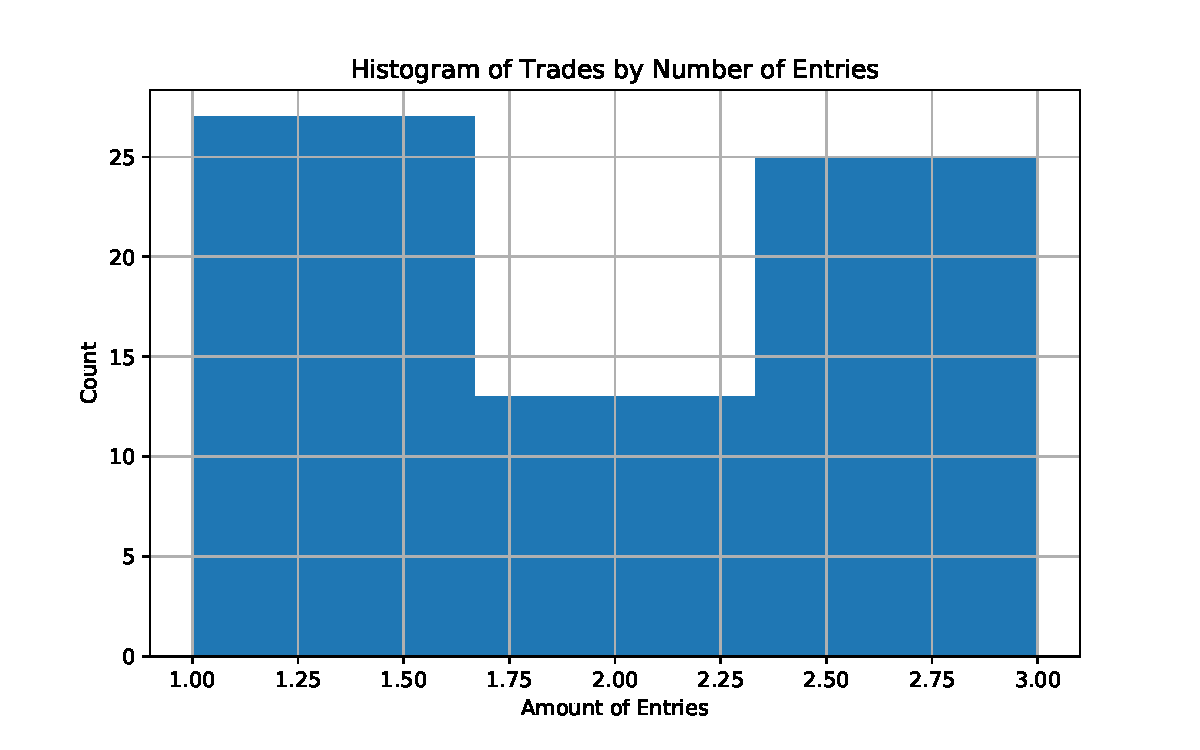
\includegraphics[width=\textwidth]{prog_entry_stop_win_lim3_hist.pdf}
	\caption{This table shows counts of the numbers of trades that had a certain amount of entries. For example, it says that around 27 trades had only 1 entry, and that around 25 trades had 3 entries (fist entry and 2 adds).}
	\label{hist_strat_2}
	\end{figure}

\pagebreak

\section{Strategy 3: 30 Min. Window Until 11, 5\% Stop Win Relative to Average Cost, Unlimited Entries }


\begin{table}
\caption{Performance of Strategy 3: 30 Min. Window Until 11, 5\% Stop Win Relative to Average Cost, Unlimited Entries}
\center{Overall}
\\[2ex]
\begin{tabular}{lcccc}
\hline
         &  0.1   &  0.9   & median & average   \\
\midrule
\midrule
constant & 0.0177 & 0.0500 & 0.0500 & 0.0440    \\
         & (inf)  & (inf)  & (inf)  & (0.0022)  \\
N        & 66     & 66     & 66     & 66        \\
Win rate & 0.95   & 0.95   & 0.95   & 0.95      \\
\hline
\end{tabular}

\center{Winners}
\\[2ex]
\begin{tabular}{lcccc}
\hline
         &  0.25  &  0.75  & median & average   \\
\midrule
\midrule
constant & 0.0500 & 0.0500 & 0.0500 & 0.0473    \\
         & (inf)  & (inf)  & (inf)  & (0.0012)  \\
N        & 63     & 63     & 63     & 63        \\
Win rate & 0.95   & 0.95   & 0.95   & 0.95      \\
\hline
\end{tabular}

\center{Losers}
\\[2ex]
\begin{tabular}{lcccc}
\hline
          &  0.25  &  0.75  & median & average   \\
\midrule
\midrule
constant  & 0.0075 & 0.0435 & 0.0258 & 0.0256    \\
          & (nan)  & (nan)  & (nan)  & (0.0104)  \\
N         & 3      & 3      & 3      & 3         \\
Loss rate & 0.05   & 0.05   & 0.05   & 0.05      \\
\hline
\end{tabular}
\label{tab_strat_3}
\end{table}

The next strategy I looked at was a `windowed' version of the baseline: all trades had to be exited within 30 minutes of being entered. Entries and stop wins occur as in the baseline. 

\textbf{The weighted expected return is 5\%}, but this again is driven by a single trade with 20 adds. This strategy has a slightly higher win percentage, 95\%, than the baseline. That being said, I would say the performance of this strategy is not significantly different than the baseline: if you have unlimited adds and a stop win, it is just as profitable to exit after 30 minutes as it is to exit at 11 am. 

\begin{figure}
	\center{Histogram of Trades by Number of Entries for 30 Min. Window Until 11, 5\% Stop Win Relative to Average Cost, Unlimited Entries}
	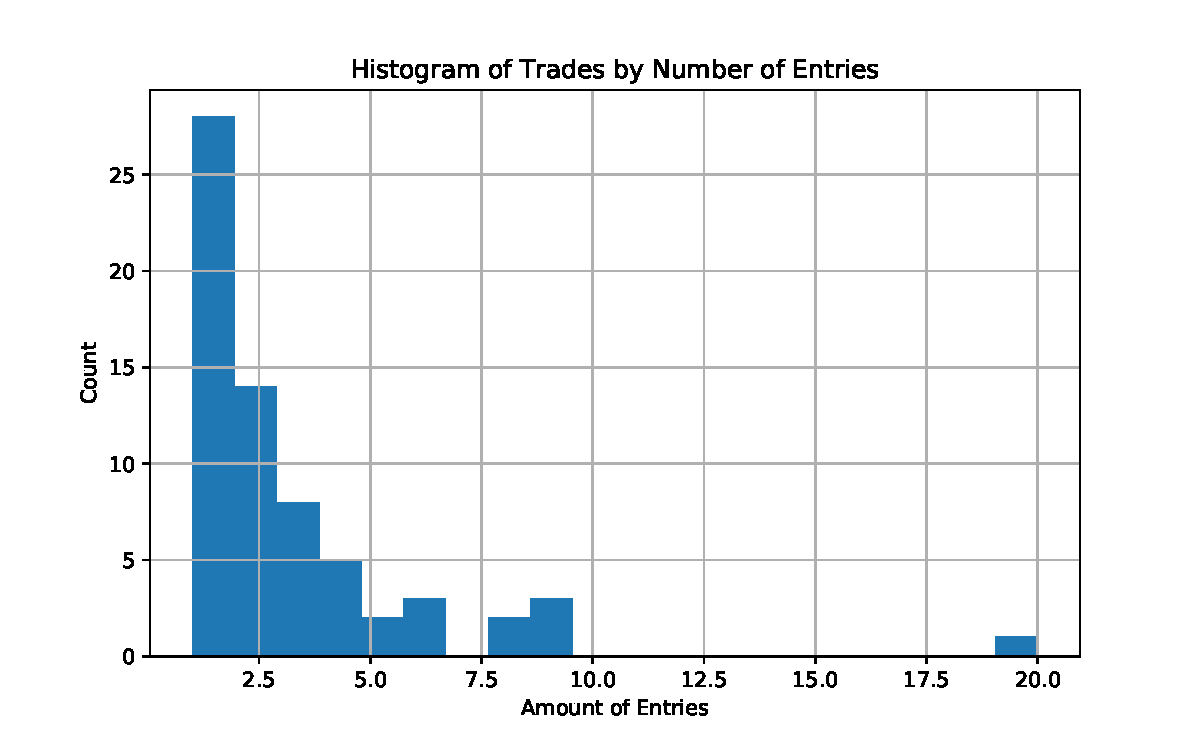
\includegraphics[width=\textwidth]{prog_entry_w30_stop_win_hist.pdf}
	\caption{This table shows counts of the numbers of trades that had a certain amount of entries. For example, it says that around 27 trades had only 1 entry, and that around 3 trades had 9 entries (fist entry and 8 adds).}
	\label{hist_strat_3}
	\end{figure}

\pagebreak

\section{Strategy 4: 30 Min. Window Until 11, Max 3 Entries 5\% Stop Win Relative to Average Cost}


\begin{table}
\caption{Performance of Strategy 4: 30 Min. Window Until 11, Max 3 Entries 5\% Stop Win Relative to Average Cost}
\center{Overall}
\\[2ex]
\begin{tabular}{lcccc}
\hline
         &   0.1   &  0.9   & median & average   \\
\midrule
\midrule
constant & -0.0258 & 0.0500 & 0.0500 & 0.0256    \\
         & (inf)   & (inf)  & (inf)  & (0.0100)  \\
N        & 66      & 66     & 66     & 66        \\
Win rate & 0.88    & 0.88   & 0.88   & 0.88      \\
\hline
\end{tabular}

\center{Winners}
\\[2ex]
\begin{tabular}{lcccc}
\hline
         &  0.25  &  0.75  & median & average   \\
\midrule
\midrule
constant & 0.0500 & 0.0500 & 0.0500 & 0.0470    \\
         & (inf)  & (inf)  & (inf)  & (0.0013)  \\
N        & 58     & 58     & 58     & 58        \\
Win rate & 0.88   & 0.88   & 0.88   & 0.88      \\
\hline
\end{tabular}

\center{Losers}
\\[2ex]
\begin{tabular}{lcccc}
\hline
          &  0.25  &  0.75  &  median  & average   \\
\midrule
\midrule
constant  & 0.0433 & 0.1300 & 0.0592   & 0.1300    \\
          & (nan)  & (nan)  & (0.0829) & (0.0606)  \\
N         & 8      & 8      & 8        & 8         \\
Loss rate & 0.12   & 0.12   & 0.12     & 0.12      \\
\hline
\end{tabular}
\label{tab_strat_4}
\end{table}

And finally I looked at a variant of the above strategy in which a maximum of 3 entries were allowed. This strategy has a \textbf{weighted return of only 1\%}, and otherwise performs similarly but slightly worse than the other three strategies.

If we want to execute a trade with a maximum of 3 entires, I think it is better to not use a trade window. 

\begin{figure}
	\center{Histogram of Trades by Number of Entries for 30 Min. Window Until 11, Max 3 Entries 5\% Stop Win Relative to Average Cost}
	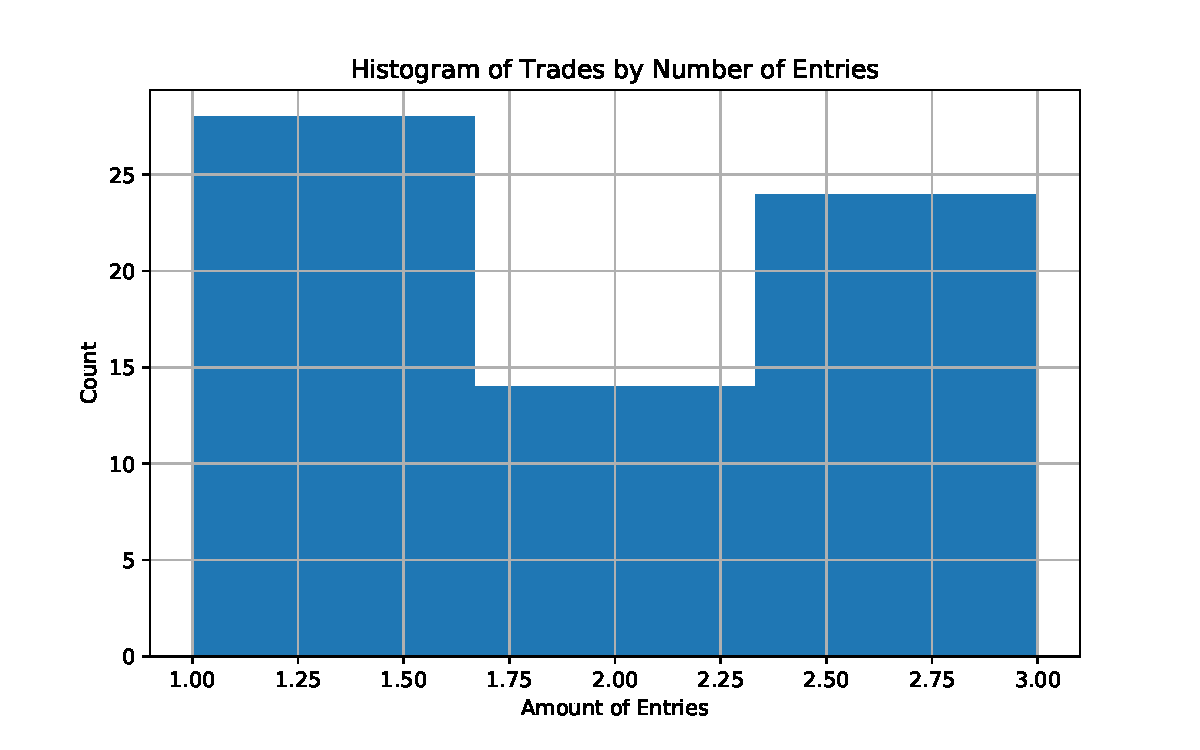
\includegraphics[width=\textwidth]{prog_entry_w30_stop_win_lim3_hist.pdf}
	\caption{This table shows counts of the numbers of trades that had a certain amount of entries. For example, it says that around 27 trades had only 1 entry, and that around 24 trades had 3 entries (fist entry and 2 adds).}
	\label{hist_strat_4}
	\end{figure}

\end{document}